%
% loesung.tex -- Beispiel-File für die Beschreibung der Loesung
%
% (c) 2020 Prof Dr Andreas Müller, Hochschule Rapperswil
%
\section{Realisierung
  \label{steps:section:loesung}}
\rhead{Realisierung}
Schrittweitensteuerungen lassen sich auf vielseitige Art und Weise realisieren,
zwei Varianten davon werden nun näher vorgestellt.

\subsection{Simple Schrittweitensteuerung mit konstannter Testschrittweite
  \label{steps:subsection:simplestep}}
Eine Möglichkeit zur Realisierung einer simplen Schrittweitensteuerung ist es, einen fixen Testschritt zu machen,
daraus eine Fehlerschätzung zu generieren, woraus sich dann eine der Kurve angepasste Schrittweite bestimmen lässt.
Die Funktionsweise dieser Methode wird nun anhand der Wahrscheinlichkeitsfunktion der Standardnormalverteilung vorgeführt.
Für die Wahrscheinlichkeitsfunktion existiert zwar keine analytische Lösung,
doch sie lässt sich aus der Wahrscheinlichkeitdichtefunktion
\[
  \varphi(x)=\frac{1}{\sqrt{2\pi}\sigma}\mathrm{e}^{-\frac{(x-\mu)^2}{2 \sigma}}\;|\mu=0,\sigma=1
\]
berechnen:
\[
  F(x)=\int_{-\infty}^{x} \varphi (\tilde{x}) \cdot \mathrm{d} \tilde{x}
\]
Damit die Funktion mittels gängiger Methoden der Differenzialrechnung analysiert werden kann,
wird die Integralfunktion in eine Differenzialgleichung umgewandelt:
\[
  F(x)'=\varphi(x)\;|F(-\infty)=0
\]
In folgendem Beispiel zur Abbildung ~\ref{buch:steps:examplessc} wurde bei $x_0=-7$ mit Startwert $F(-7)=\tilde{F}_0=0$ begonnen.
Dabei wird für den Schritt $n$ die Steigung ($\varphi$) am Punkt $x_{n-1}, \tilde{F}_{n-1}$ (in Abbildung oranger Punkt mit rotem Kreuz) berechnet.
Damit wird ein Eulerschritt mit der Testschrittweite $h_{test}=2$ (In Abbildung als schwarzer Balken oberhalb der x-Achse) gemacht
$\implies P_{test}=(x_n+h_{test}, \tilde{F}_n+\varphi(x_n, \tilde{F}_n)$.
Nun wird auch an diesem Punkt (In Abbildung als einsames rotes Kreuz am oberen Ende der Grafik) die Steigung ermittelt.
Sind die beiden Steigungen am Start und am Endpunkt des Testschrittes ziemlich ähnlich, wird davon ausgegangen,
dass die Kurve in diesem Bereich nur wenig ihre Richtung ändert und deshalb eine grosse Schrittweite gewählt werden darf.
Ist der Unterschied (Abbildung, untere Grafik, Differenz zwischen phi(start), phi(test)) etwas grösser,
wird die Schrittweite (In Abbildung roter Balken innerhalb der Testschrittweite) etwas kleiner gewählt.
Konkret berechnet sich in diesem Beispiel die zu wählende Schrittweite wie folgt:
\[
  h=\frac{h_{test}}{|\varphi(x_n, \tilde{F}_n)-\varphi(P_{test})|\cdot q_{factor}}\; |q_{factor}=20
\]
Wobei die Schrittweite nach oben zusätzlich durch die Testschrittweite begrenzt wird,
da der Verlauf der Kurve jenseits des Testpunktes noch nicht bekannt ist.
Auch eine Division durch Null muss abgefangen werden, falls die Steigung in beiden Punkten identisch ist,
wobei dann die maximale Schrittweite $h=h_{test}$ gewählt werden darf.
Mit der nun ermittelten Schrittweite wird ein Runge-Kutta-Schritt (4. Ordnung) gemacht,
wobei einer der Koeffizienten ($k_1$) bereits beim Testschritt ermittelt worden ist.

Dieses Verfahren ist zwar in der Lage, die Schrittweite zu verkleinern, falls mit der Testschrittweite ein zu grosser Fehler resultieren würde,
doch über den Fehler des gemachten Schrittes ist dann am Ende nichts bekannt.
Eine weitere Schwäche dieses konstannten Testschrittes ist, dass bereits sehr kleine Schritte gewählt werden,
sobald der Testschritt eine andere Steigung ertastet, obwohl der "Knick" der Kurve noch genügend weit entfernt wäre.

\begin{figure}
  \centering
  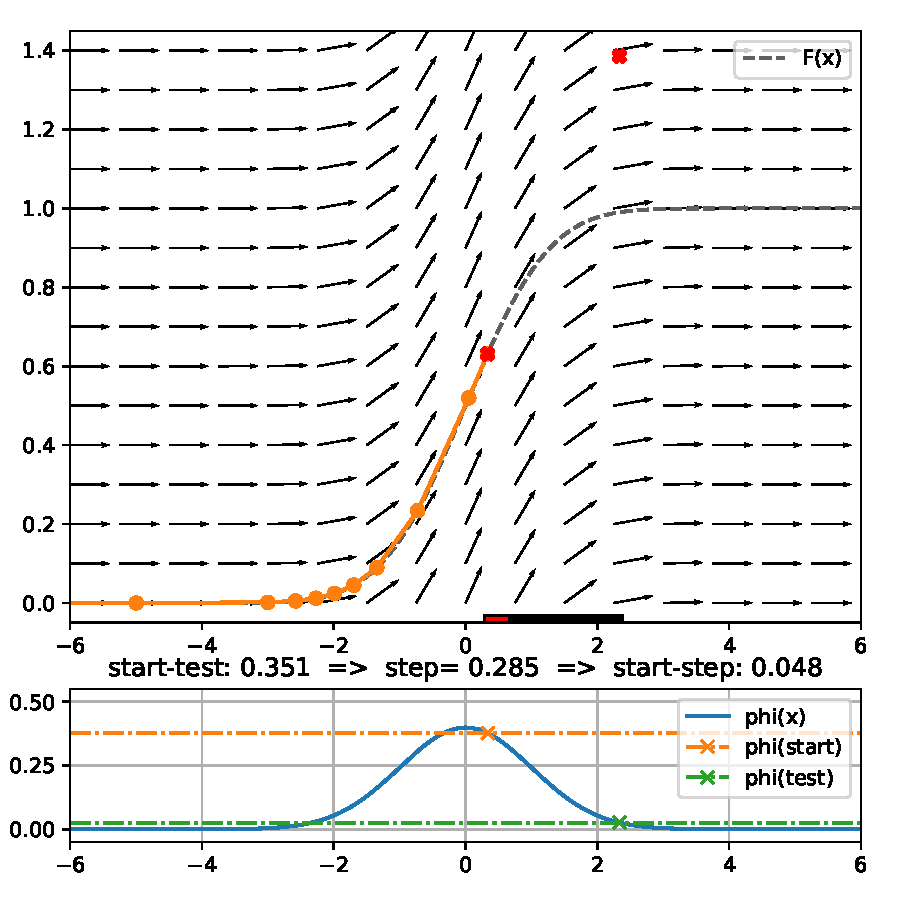
\includegraphics[width=0.5\textwidth]{papers/steps/img/ssc.pdf}
  \caption{Berechnung der Wahrscheinlichkeitsfunktion $F(x)$ der Standardnormalverteilung aus dessen Dichtefunktion
    (oben mit Pfeilen, unten als Funktion phi(x)) mit einer einfachen Schrittweitensteuerung
    \label{buch:steps:examplessc}}
\end{figure}

\subsection{Schrittweitensteuerung mit Fehlberg
  \label{steps:subsection:fehlberg}}
Eine andere Möglichkeit zur Realisierung einer Schrittweitensteuerung ist die Methode mit Fehlberg
\cite{steps:Numerische-Mathematik}.
Dabei wird der Fehler des aktuellen Schrittes anhand der Differenz zweier unterschiedlichen, parallelen
Runge-Kutta Schritten geschätzt. Durch geschickte Kombination dieser beiden Schritte
lässt sich der Mehrrechenaufwand dazu aber merklich reduzieren, was in der Literatur als "einbetten" bezeichnet wird.
In folgendem Beispiel wird gezeigt, wie ein vierstufiger Runge-Kutta Schritt 4. Ordnung in ein sechsstufiger Schritt 5. Ordnung eingebettet wird.
Dabei werden zuerst alle Koeffizienten berechnet, welche für den Schritt 4. Ordnung nötig sind:
\begin{align*}
  k_1 & =f(x_j, u_j)                                                                           \\
  k_2 & =f(x_j + \frac{2}{9}h, u_j+\frac{2}{9}hk_1)                                            \\
  k_3 & =f(x_j + \frac{1}{3}h, u_j+\frac{1}{12}hk_1+\frac{1}{4}hk_2)                           \\
  k_4 & =f(x_j + \frac{3}{4}h, u_j+\frac{69}{128}hk_1-\frac{243}{128}hk_2+\frac{135}{64}hk_3)  \\
  k_5 & =f(x_j + h, u_j-\frac{17}{12}hk_1+\frac{27}{4}hk_2-\frac{27}{5}hk_3+\frac{16}{15}hk_4)
\end{align*}
Daraus kann nun eine erste Schätzung für den Punkt am Schrittende gemacht werden:
\[
  u_{j+1} =u_j +h\cdot(\frac{1}{9}k_1+\frac{9}{20}k_3+\frac{16}{45}k_4+\frac{1}{12}k_5)
\]
Mit einem weiteren Koeffizienten
\[
  k_6 =f(x_j + \frac{5}{6}h, u_j+\frac{65}{432}hk_1-\frac{5}{16}hk_2+\frac{13}{16}hk_3+\frac{4}{27}hk_4+\frac{5}{144}hk_5)
\]
lässt sich nun eine zweite Schätzung für den Endpunkt berechnen:
\[
  \hat{u}_{j+1} =u_j+h\cdot(\frac{47}{450}hk_1+\frac{12}{25}hk_3+\frac{32}{225}hk_4+\frac{1}{30}hk_5+\frac{6}{25}hk_6)
\]
Den lokalen Fehler des Schrittes lässt sich nun durch den Betrag der Differenz der beiden Endpunkte schätzen.
\[
  T(x_{j+1},h)=|u_{j+1}-\hat{u}_{j+1}|=\frac{h}{300}\cdot|-2k_1+9k_3-64k_4-15k_5+72k_6|
\]
Doch da beide Schätzungen eine Linearkombination der Koeffizienten $k_1$ bis $k6$ sind,
lässt sich die Differenz auch direkt aus den Linearkombinationen ermitteln,
sodass der zweite Schätzwert $\hat{u}_{j+1}$ überflüssig wird.

Mit dieser Fehlerschätzung lässt sich nun ein Algorithmus wie in Abbildung ~\ref{buch:steps:flowchartfehlberg} steuern,
welcher die Schrittlänge kontrolliert. Falls die Schätzung des Fehlers $T(x_{j+1}, h_j)$ nun grösser ist als die erlaubte Toleranz $\varepsilon$,
wird die Schrittweite halbiert und der Schritt wiederholt.
Falls der Fehler viel kleiner ist als die erlaubte Toleranz, wird die Schrittweite für den nächsten Schritt verdoppelt.

\begin{figure}
  \centering
  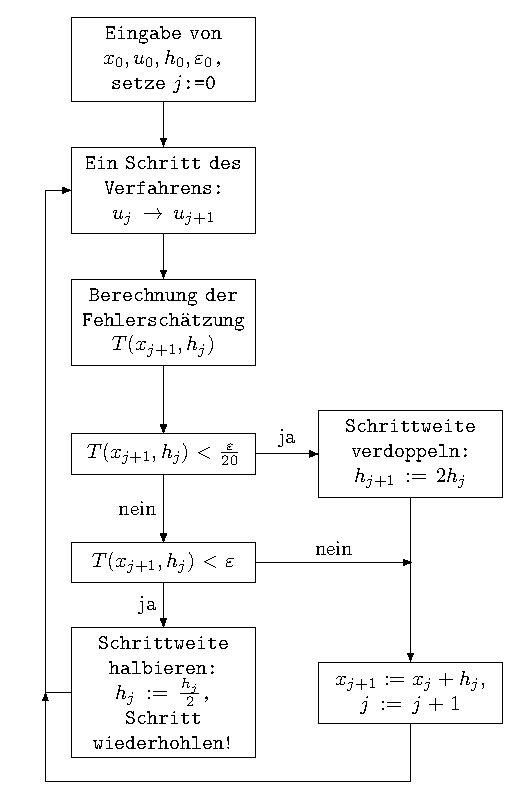
\includegraphics[width=0.5\textwidth]{papers/steps/img/Fehlberg_Flowchart.pdf}
  \caption{Algorithmus zur Schrittlängensteuerung
    \label{buch:steps:flowchartfehlberg}}
\end{figure}
